{
\chapter{Data augmentation invariance}
\label{ch:invariance}
\renewcommand{\chapterpath}{includes/invariance}
%
\begin{contributors}
    Tim C. Kietzmann supervised the work during my internship at his lab. Tim and Peter K{\"o}nig reviewed and edited the manuscripts submitted to conferences.
\end{contributors}
\begin{outreach}
    \item \textit{Learning robust visual representations using data augmentation invariance.} \textbf{Alex Hern{\'a}ndez-Garc{\'i}a}, Peter K{\"o}nig, Tim C. Kietzmann. arXiv preprint arXiv:1906.04547 \& Cognitive Computational Neuroscience (CCN), 2019 \& Workshop on Bridging AI and Cognitive Science, International Conference on Learning Representations (ICLR), 2019.
    \item \textit{Learning representational invariance instead of categorization.} \textbf{Alex Hern{\'a}ndez-Garc{\'i}a}, Peter K{\"o}nig. Workshop on pre-registration in computer vision, International Conference on Computer Vision (ICCV), 2019.
\end{outreach}
%
Deep artificial neural networks (ANNs) have borrowed much inspiration from neuroscience and are, at the same time, the current best model class for predicting neural responses across the visual system in the brain \citep{kietzmann2019dnncompneuro, kubilius2018cornet}. Yet, despite consensus about the benefits of a closer integration of deep learning and neuroscience \citep{bengio2015dlandneuroscience, marblestone2016dlandneuroscience, richards2019dlandneuroscience}, important differences remain \citep{sinz2019dlvsbrain, geirhos2020shortcutlearning, dujmovic2020adversarial}.

Here, we investigate a representational property that is well established in the neuroscience literature on the primate visual system: the increasing robustness of neural responses to identity-preserving image transformations. While early areas of the ventral stream (V1-V2) are strongly affected by variation in object size, position, viewpoint and other factors, later levels of processing are increasingly robust to such changes, as measured first in single neurons of the inferior temporal (IT) cortex of macaques \cite{booth1998invariantitmacaque} and then in humans' \citep{quiroga2005invariantithuman, isik2013dynamics}. The cascaded achievement of invariance to such identity-preserving transformations has been proposed as a key mechanism for robust object recognition \citep{dicarlo2007untangling, tacchetti2018invariance}.

Learning such invariant representations has been a desired objective since the early days of artificial neural networks \citep{simard1992daug}. Accordingly, a myriad of techniques have been proposed to attempt to achieve tolerance to different types of transformations (\citet{cohen2016groupequivcnns} briefly reviewed some of these efforts). Interestingly, recent theoretical work \citep{achille2018emergence} has shown that invariance to ``nuisance factors'' should naturally emerge from the optimisation process of deep models that minimise the information of the representations about the inputs, while retaining the minimum information about the target, as proposed by \citet{tishby2015infobottleneck} in the information bottleneck principle.

Nevertheless, artificial neural networks are still not robust to identity-preserving transformations, including simple image translations \citep{zhang2019convolutions}. A remarkable extreme example are adversarial attacks \citep{szegedy2013adversarial}, in which small changes, imperceptible to the human brain, can alter the classification output of the network. Extending this line of research, we used data augmentation as a framework to generate the transformations to which vision models should be invariant to, according to visual perception and biological vision. As a first contribution, we propose a simple metric, \textit{data augmentation invariance score}, to measure the invariance of neural networks to identity-preserving transformations.

Second, inspired by the increasing invariance observed along the primate ventral stream of the visual cortex, we here propose \textit{data augmentation invariance}, a simple, yet effective and efficient mechanism to improve the robustness of the representations: we include an additional contrastive term in the objective function that encourages the similarity between augmented examples within each batch. We will argue that this objective encodes a useful inductive bias that exploits prior knowledge from visual perception and biological vision.

Finally, we explore the possibility of fully replacing the categorisation objective that is commonly used to train neural networks for classification, the categorical cross-entropy, by objective functions purely based on invariance learning.

\section{Invariance score}
\label{sec:invariance-eval}
To measure the invariance of the learnt features under the influence of identity-preserving image transformations we compare the activations of a given image with the activations of an augmented version of the same image. 

Consider the activations of an input image $x$ at layer $l$ of a neural network, which can be described by a function $f^{(l)}(x) \in \mathbb{R}^{D^{(l)}}$. We can define the distance between the activations of two input images $x_{i}$ and $x_{j}$ by their mean squared difference:

\begin{equation}
\label{eq:invariance-mse}
 d^{(l)}(x_{i}, x_{j}) = \frac{1}{D^{(l)}}\sum_{k=1}^{D^{(l)}}(f_{k}^{(l)}(x_{i}) - f_{k}^{(l)}(x_{j}))^2
\end{equation}

Following this, we are interested in the mean squared distance between $f^{(l)}(x_i)$ and a randomly sampled transformation of $x_i$, that is $d^{(l)}(x_{i}, G(x_{i}))$. $G(x)$ refers to the stochastic function that transforms the input images according to a pre-defined, parameterised data augmentation scheme.

In order to assess the similarity between the activations of an image $x_i$ and of its augmented versions $G(x_{i})$ we normalise it by the average similarity in the (test) set. We define the \textit{data augmentation invariance score} $S_{i}^{(l)}$ of image $x_i$ towards the transformation $G(x)$ at layer $l$ of a model, with respect to a data set of size $N$, as follows:

\begin{equation}
\label{eq:invariance-invariance}
 S_{i}^{(l)} = 1 - \frac{d^{(l)}(x_{i}, G(x_{i}))}{\frac{1}{N}\sum_{j=1}^{N}d^{(l)}(x_{i}, x_{j})}
\end{equation}

Note that the invariance $S_{i}^{(l)}$ takes the maximum value of 1 if the activations of $x_{i}$ and its transformed version $G(x_{i})$ are identical, and the value of 0 if the distance between transformed examples, $d^{(l)}(x_{i}, G(x_{i}))$ (numerator), is equal to the average distance in the set (denominator).

\subsection{Learning objective}
\label{sec:invariance-daug_invariance}
Most ANNs trained for object categorisation are optimised through mini-batch stochastic gradient descent (SGD), that is the weights are updated iteratively by computing the loss of a batch $\mathcal{B}$ of examples, instead of the whole data set at once. The models are typically trained for a number of \textit{epochs} $E$ which is a whole pass through the entire training data set of size $N$. That is, the weights are updated $K=\frac{N}{|\mathcal{B}|}$ times each epoch.

Data augmentation introduces variability into the process by performing a different, stochastic transformation of the data every time an example is fed into the network. However, with standard data augmentation, the model has no information about the \textit{identity} of the images. In other words, different augmented examples, seen at different epochs, separated by $\frac{N}{|\mathcal{B}|}$ iterations on average, correspond to the same seed data point. This information is potentially valuable and useful to learn better representations. For example, in biological vision, the high temporal correlation of the stimuli that reach the visual cortex may play a crucial role in the creation of robust connections \citep{becker1999temporalstability, kording2004complexcells, wyss2006temporalstability}. However, this is generally not exploited in supervised settings. In semi-supervised learning, where the focus is on learning from fewer labelled examples, data augmentation has been used as a source of variability together with dropout or random pooling, among others \citep{laine2016ssl}.

In order to make use of this information and improve the robustness, we first propose \textit{in-batch} data augmentation by constructing the batches with $M$ transformations of each example---\citet{hoffer2019batchaugmentation} recently discussed a similar idea. Additionally, we propose a new objective function that accounts for the invariance of the feature maps across multiple image samples. Considering the difference between the activations at layer $l$ of two images, $d^{(l)}(x_{i}, x_{j})$, defined in Equation~\ref{eq:invariance-mse}, we define the \textit{data augmentation invariance} loss at layer $l$ for a given batch $\mathcal{B}$ as follows:

\begin{equation}
\label{eq:invariance-data_aug_inv}
 \mathcal{L}_{inv}^{(l)} = \frac{\sum_{k}\frac{1}{|\mathcal{S}_{k}|^2}\sum_{x_i, x_j \in \mathcal{S}_{k}}d^{(l)}(x_{i}, x_{j})}{\frac{1}{|\mathcal{B}|^2}\sum_{x_i, x_j \in \mathcal{B}}d^{(l)}(x_{i}, x_{j})}
\end{equation}
%
where $\mathcal{S}_{k}$ is the set of samples in the batch $\mathcal{B}$ that are augmented versions of the same seed sample $x_k$. This loss term intuitively represents the average difference of the activations between the sample pairs that correspond to the same source image, relative to the average difference of all pairs. A convenient property of this definition is that $\mathcal{L}_{inv}$ does not depend on either the batch size or the number of in-batch augmentations $M=|\mathcal{S}_{k}|$. Furthermore, it can be efficiently implemented using matrix operations. Our data augmentation invariance can be seen as a contrastive loss \citep{hadsell2006contrastive}, since the aim is to bring closer the representations of related examples---transformations of the same source image---and push apart the representations from other examples.

In order to simultaneously achieve certain representational invariance at $L$ layers of the network and high object recognition performance at the network output, we define the total loss as follows:

\begin{equation}
 \mathcal{L} = (1 - \alpha)\mathcal{L}_{obj} + \sum_{l=1}^{L}\alpha^{(l)}\mathcal{L}_{inv}^{(l)}
\end{equation}
%
where $\alpha = \sum_{l=1}^{L}\alpha^{(l)}$ and $\mathcal{L}_{obj}$ is the loss associated with the object recognition objective, typically the cross-entropy between the object labels and the output of a softmax layer. For all the experiments presented in this chapter, we set $\alpha=0.1$ and distributed the coefficients across the layers according to an exponential law, such that $\alpha^{(l=L)}= 10\alpha^{(l=1)}$. This aims at simulating a probable response along the ventral visual stream, where higher regions are more invariant than the early visual cortex\footnote{It is beyond the scope of this study to analyse the sensitivity of the hyperparameters $\alpha^{(l)}$, but we did not observe a significant impact in the classification performance by using other distributions.}.

\subsection{Architectures and data sets}
\label{sec:invariance-arch-and-data}
As test beds for our hypotheses and proposal we trained three neural network architectures: all convolutional network, All-CNN-C \citep{springenberg2014allcnn}; wide residual network, WRN-28-10 \citep{zagoruyko2016wrn}; and DenseNet-BC \citep{huang2017densenet}. All three architectures have been widely used in the deep learning literature, including our experiments in Chapter~\ref{ch:daugreg}, where the details can be consulted. They provide generality of the results, as they have distinctive architectural characteristics: only convolutional layers, residual blocks and dense connectivity, respectively.

We trained the three architectures on the highly benchmarked data set for object recognition CIFAR-10 \citep{krizhevsky2009cifar}. Additionally, in order to test our proposal on higher resolution images and a larger number of classes, we also trained All-CNN and WRN on the \textit{tiny} ImageNet data set, a subset of ImageNet \citep{russakovsky2015imagenet} with 100,000 64x64 training images that belong to 200 classes. All models were trained using the \textit{heavier} data augmentation scheme as defined in Section~\ref{sec:daugreg-methods_data}, which consists of affine transformations, contrast adjustment and brightness adjustment.

For the models trained on CIFAR-10, the training hyperparameters---learning rate, decay, number of epochs, etc.---were set as in the original papers, except that, following the conclusions from Chapter~\ref{ch:daugreg}, we did not use explicit regularisation---weight decay and dropout---since comparable performance is obtained without them if data augmentation is used. For all three architectures, we performed $M=|\mathcal{S}_{k}|=8$ augmentations per image in the batch, while keeping the real batch size as in the original papers.

On tiny ImageNet, All-CNN included three additional layers and was trained for 150 epochs, with batch size 128 and initial learning rate 0.01 decayed by 0.1 at epochs 100 and 125. We included $M=8$ augmentations per image in the batches. WRN was trained for 50 epochs, with batch size 32 and initial learning rate 0.01 decayed by 0.2 at epochs 30 and 40. To train WRN with data augmentation invariance, we performed $M=4$ augmentations per image. In all cases, the models were trained with stochastic gradient descent with Nesterov momentum 0.9. 

Note that the hyperparameters were fine-tuned for the original papers by training only with the standard categorical cross-entropy and with standard epoch-wise data augmentation. Therefore, they were likely suboptimal for our proposed data augmentation invariance. However, our aim was not achieving the best possible classification performance, but rather demonstrate the suitability of data augmentation invariance and analyse the learnt representations.

The invariance loss defined in Equation~\ref{eq:invariance-data_aug_inv} was computed after the ReLU activation of each convolutional layer for All-CNN, at the output of each residual block for WRN, and after the first convolution and the output of each dense block for DenseNet.

\section{Results}
\label{sec:invariance-results}
The first contribution of this chapter is to empirically test in how far convolutional neural networks trained for object categorisation produce invariant representations under the influence of identity-preserving transformations of the input images. Figures~\ref{fi:invariance-invariance_allcnn}--\ref{fi:invariance-invariance_densenet} show the invariance scores, as defined in Equation~\ref{eq:invariance-invariance}, across the network layers. Since we do not compute the invariance score at every single layer of the architectures, the numbering of the layers simply indicate increasing depth in the hierarchy (see Section~\ref{sec:invariance-arch-and-data} for the details). The red boxes correspond to the baseline models and the blue boxes to the models trained with our data augmentation invariance objective.

\begin{figure}[ht]
  \begin{center}
    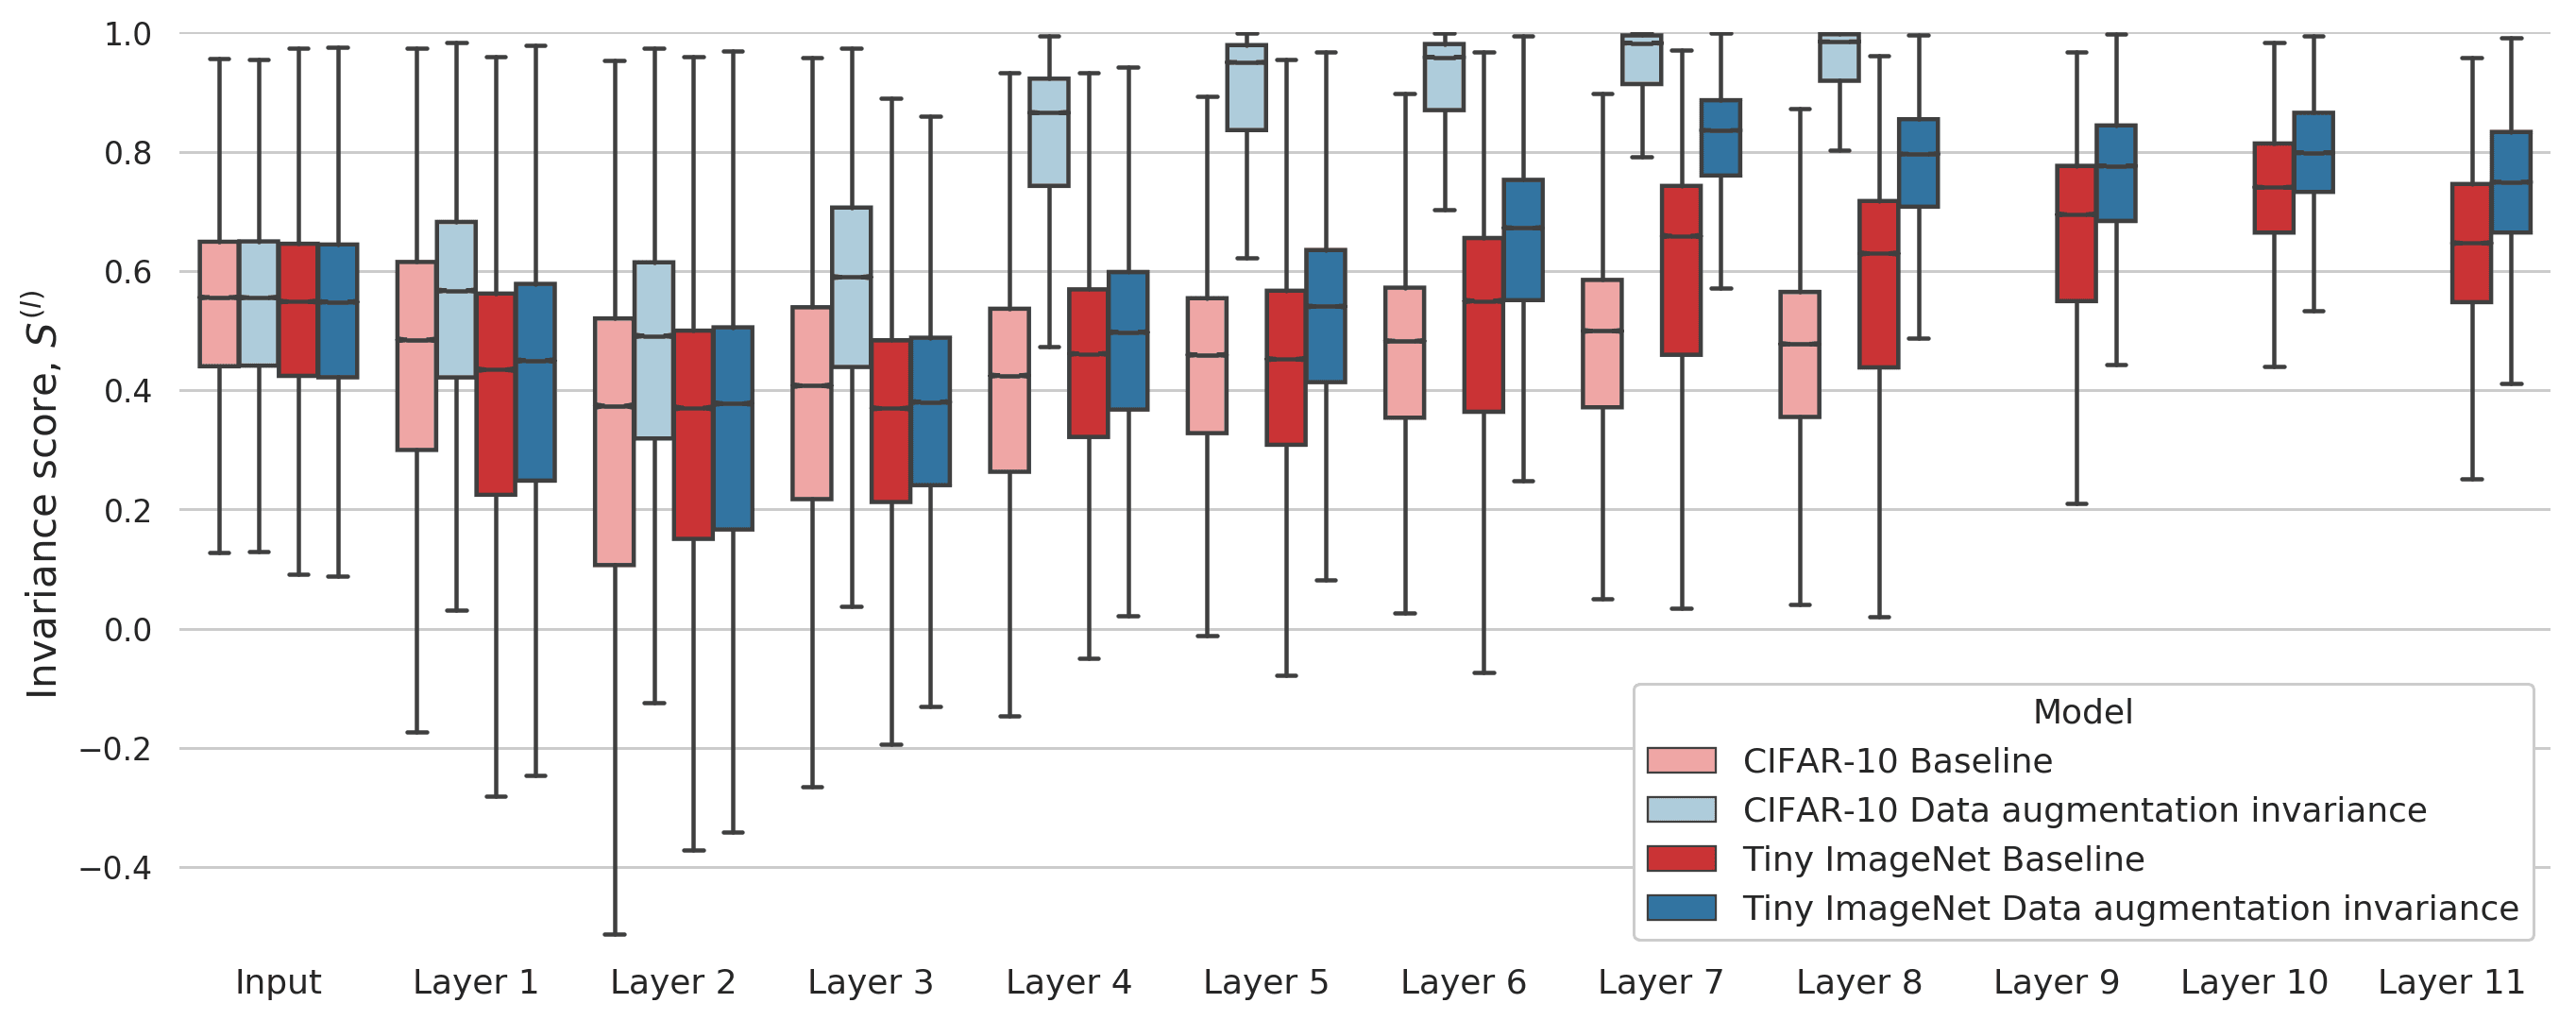
\includegraphics[width = \linewidth]{\imgpath/invariance_allcnn.png}
  \end{center}
  \caption{All-CNN: distribution of the invariance score at each layer of the baseline model and the model trained data augmentation invariance (higher is better).}
  \label{fi:invariance-invariance_allcnn}
\end{figure}

\begin{figure}[ht]
  \begin{center}
    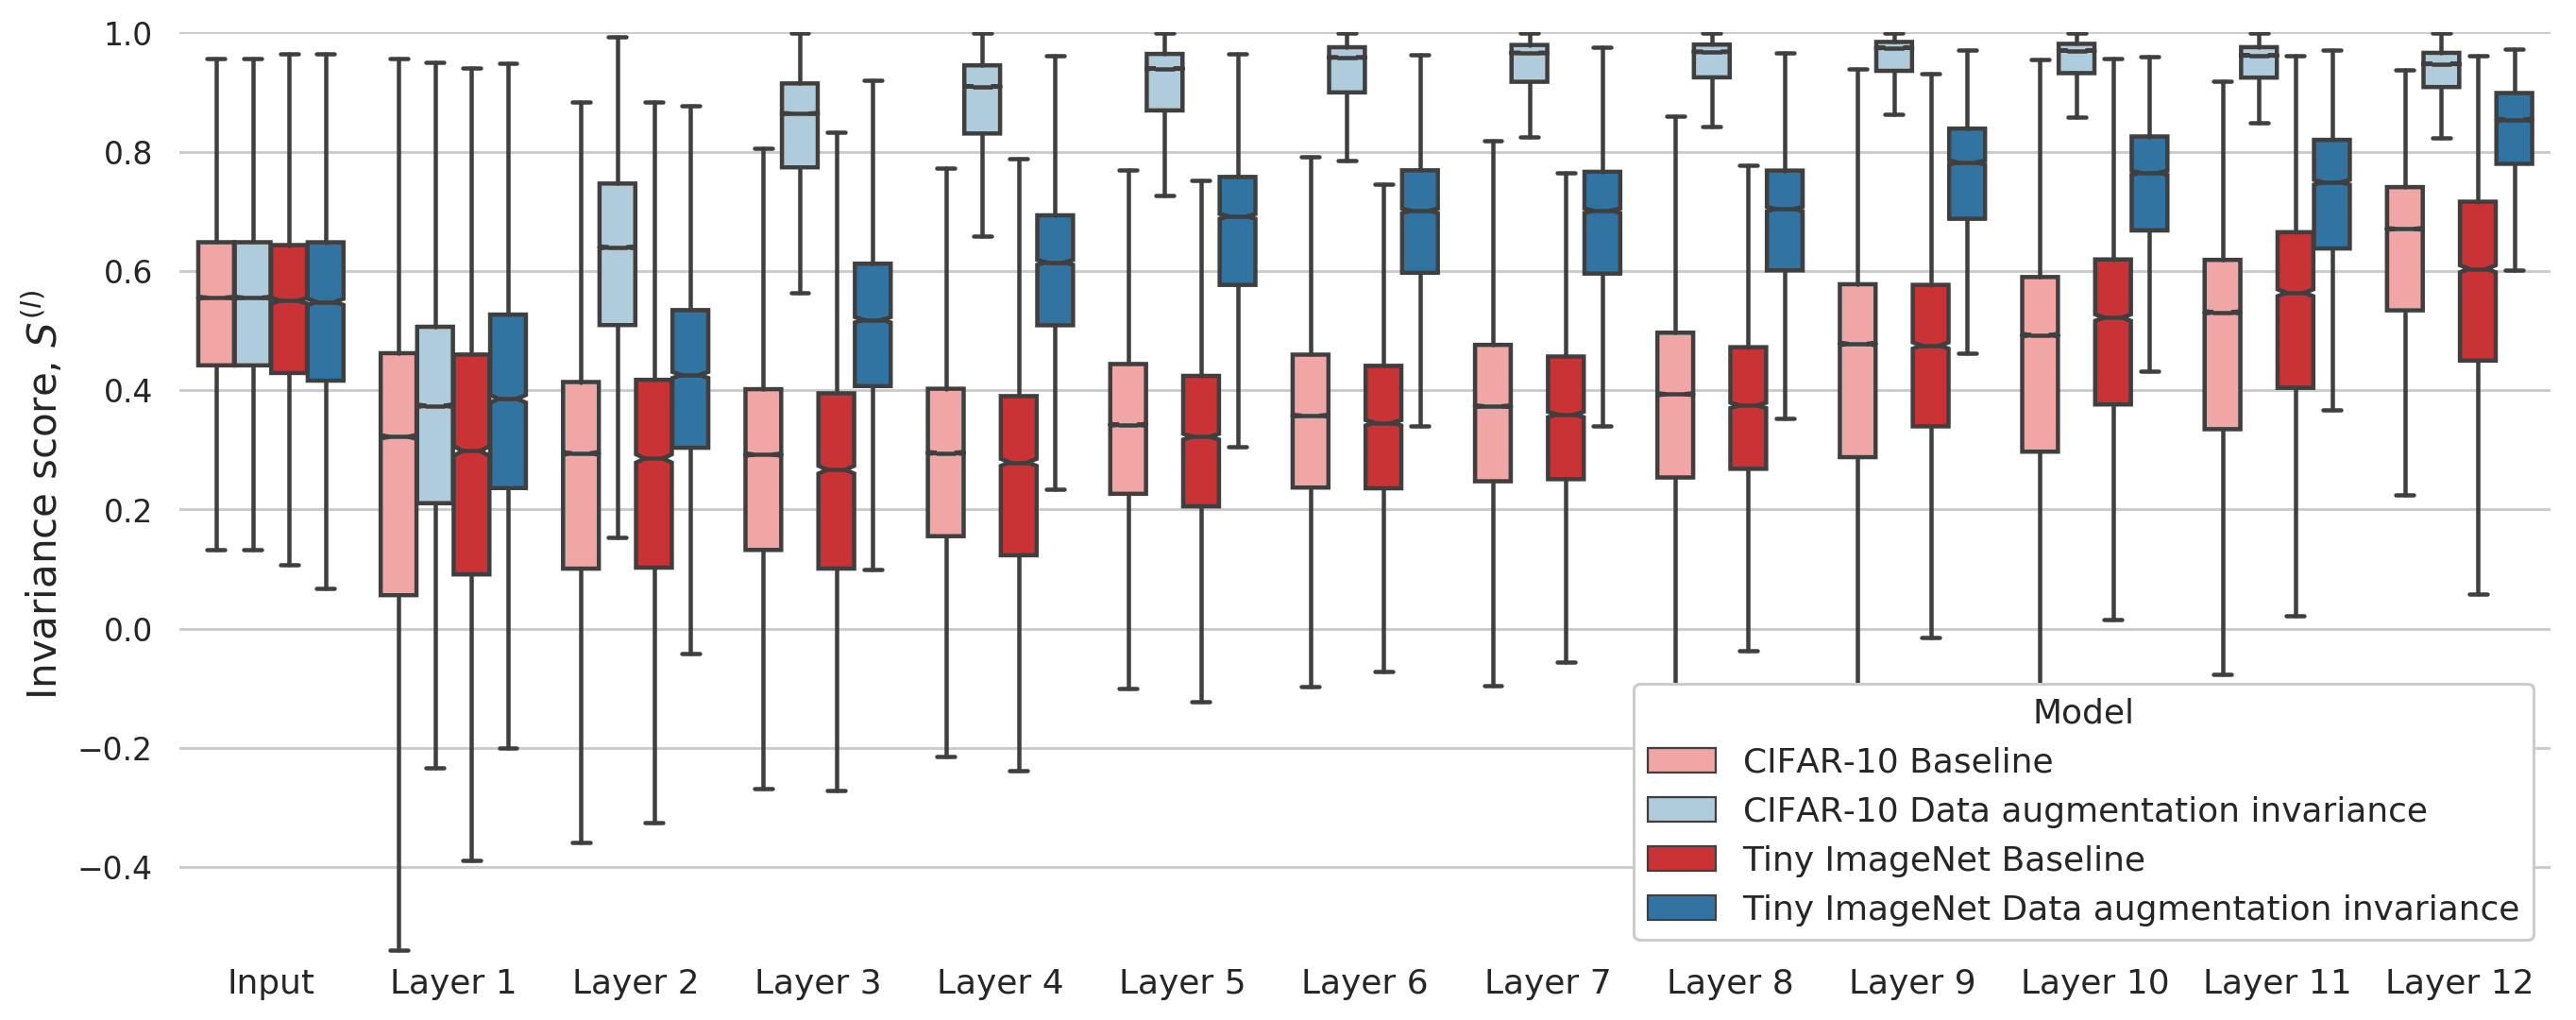
\includegraphics[width = \linewidth]{\imgpath/invariance_wrn.png}
  \end{center}
  \caption{WRN: distribution of invariance score at each layer of the baseline model and the model trained data augmentation invariance (higher is better).}
  \label{fi:invariance-invariance_wrn}
\end{figure}

\begin{figure}[ht]
  \begin{center}
    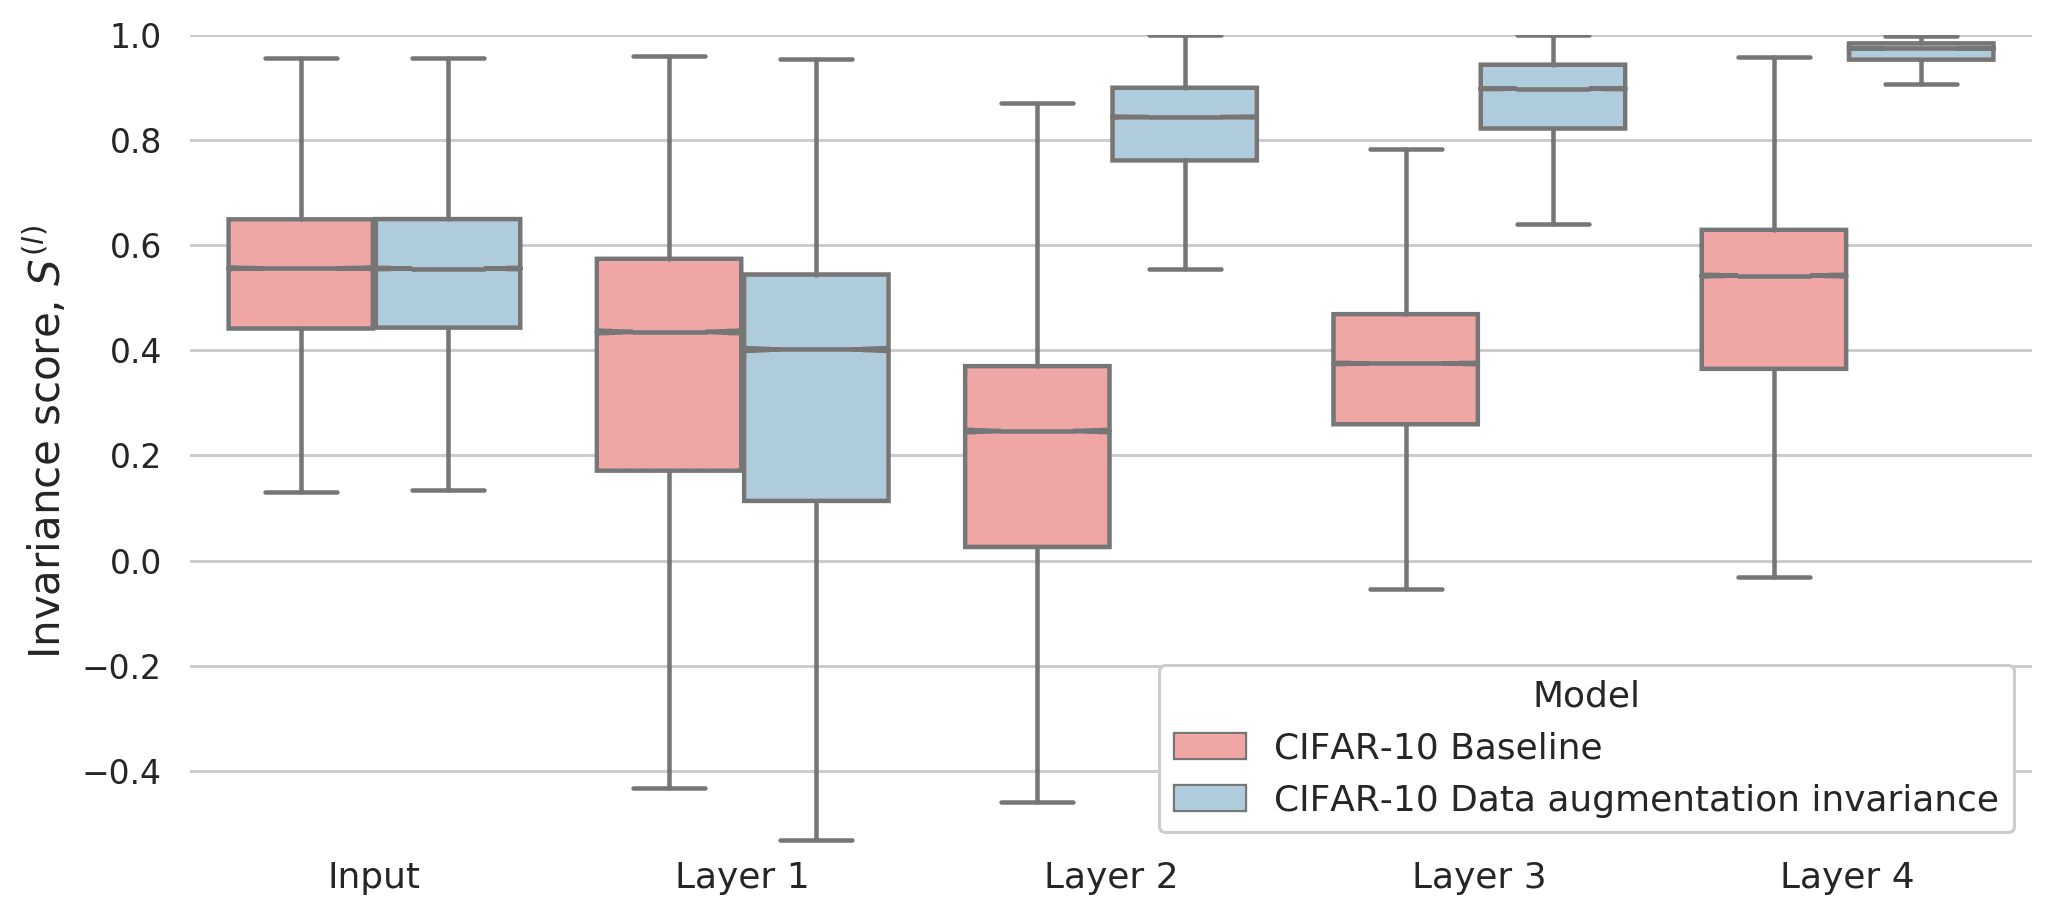
\includegraphics[width = \linewidth]{\imgpath/invariance_densenet.png}
  \end{center}
  \caption{DenseNet: distribution of invariance score at each layer of the baseline model and the model trained data augmentation invariance (higher is better).}
  \label{fi:invariance-invariance_densenet}
\end{figure}

The distributions of the invariance score shown in the figures were computed using the test partitions of the data. For each image, we performed five random transformations using as parameters the values at exactly half of the range used for training (see Section~\ref{sec:daugreg-methods_data}). Despite the presence of data augmentation during training, which implies that the networks \textit{sees} and may learn augmentation-invariant transformations, the representations of the baseline models (red boxes) do not increase substantially beyond the invariance observed in the pixel space (left-most boxes). To illustrate this, see the images in Figure~\ref{fig:invariance-sample_images}, whose representations are all equally distant to the reference image, despite the perceptual similarity of the transformed images. 

\begin{figure}[htb]
  \begin{center}
    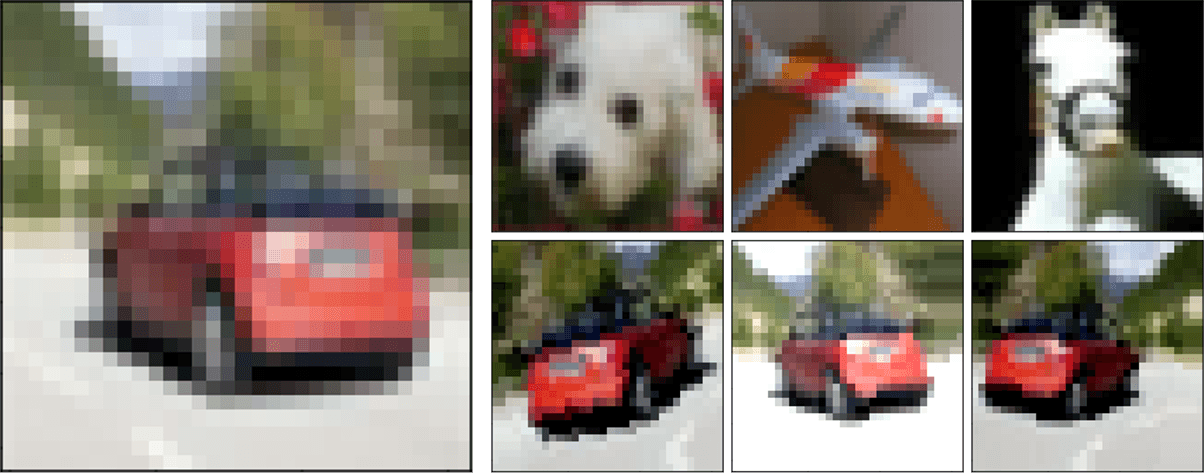
\includegraphics[width = 0.8 \linewidth]{\imgpath/sample_images.png}
  \end{center}
  \caption{The top layer representations of the six images on the right learnt by All-CNN are equally (dis)similar to the reference image (left), even though the images at the bottom row are transformations of it.}
  \label{fig:invariance-sample_images}
\end{figure}

As a solution, we have proposed a simple, label-free modification of the loss function to encourage the learning of data augmentation-invariant features. The blue boxes in Figures~\ref{fi:invariance-invariance_allcnn}--\ref{fi:invariance-invariance_densenet} show that our invariance mechanism pushed network representations to become increasingly more robust with network depth\footnote{Both All-CNN and WRN seem to more easily achieve the representational invariance on CIFAR-10 than on Tiny ImageNet. This may indicate that the complexity of the data set not only makes the object categorisation more challenging, but also the learning of invariant features.}. As discussed above, this is a well-studied property of the visual ventral stream in the primate brain. 

In order to better understand the effect of the data augmentation invariance objective, we analysed the learning dynamics of the invariance loss at each layer of All-CNN trained on CIFAR-10. In Figure~\ref{fig:dynamics}, we see that in the baseline model, the invariance loss keeps increasing over the course of training. In contrast, in the models trained with data augmentation invariance, the loss drops for all but the last layer. Perhaps unexpectedly, the invariance loss increases during the first epochs and only then starts to decrease. While further investigation is required, these two phases may correspond to the fitting and compression-diffusion phases proposed in the framework of the information bottleneck principle by \citet{shwartz2017bottleneck}. According to the authors, during the first epochs of optimisation with SGD, the model increases the information about the labels (fitting) and during the rest of training, the model reduces the information on the input (compression). However, note that \citet{saxe2019informationbottleneck} have argued that this occurs only in some cases that depend on the non-linearities.

\begin{figure}[ht]
  \begin{center}
    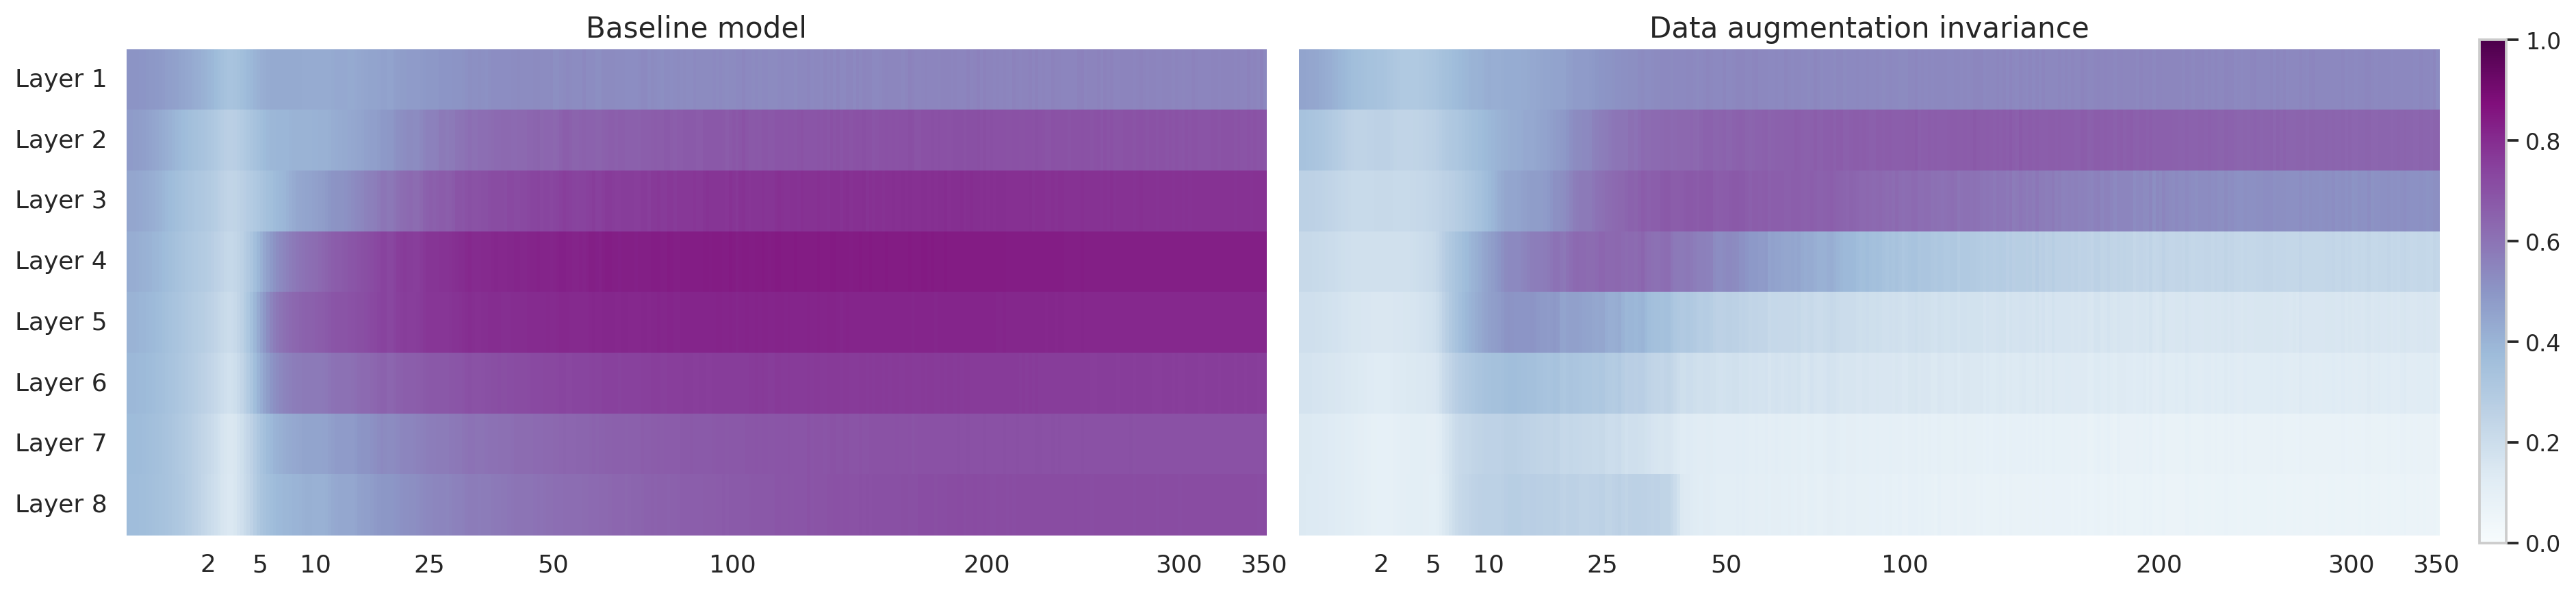
\includegraphics[width = \linewidth]{\imgpath/loss_dynamics.png}
  \end{center}
  \caption{Dynamics of the data augmentation invariance loss $\mathcal{L}_{inv}^{(l)}$ during training (lower is better). The axis of abscissas (epochs) is scaled quadratically to better appreciate the dynamics at the first epochs. The same random initialisation was used for both models.}
  \label{fig:dynamics}
\end{figure}

In terms of efficiency, adding terms to the objective function implies an overhead of the computations. However, since the pairwise distances can be efficiently computed at each batch through matrix operations, the training time was only increased by about 10 \% on average. 

Finally, as reported in Table~\ref{tab:accuracy}, the improved invariance comes at little or no cost in the categorisation performance, as the networks trained with data augmentation invariance achieved similar classification performance to the baseline model and in some cases it clearly improved it. This is remarkable as the hyperparameters used in all cases were optimised to maximise the performance in the original models, trained without data augmentation invariance. Therefore, it is reasonable to expect an improvement in the classification performance if, for instance, the batch size or the learning rate schedule are better tuned for this new learning objective. Learning increasingly invariant features could lead to more robust categorisation, as exemplified by the increased test performance observed for the All-CNN models---despite no hyperparameter tuning.

\begin{table}[tb]
  \begin{center}
    \begin{tabular}{rccccc}
	  & \multicolumn{3}{c}{CIFAR-10} & \multicolumn{2}{c}{Tiny ImageNet (acc. | top5)}          \\
      \cline{2-6} 
	                               & All-CNN & WRN   & DenseNet & All-CNN       & WRN   \\
	  Baseline                     & 91.48   & 94.58 & 94.88    & 51.09 | 73.48 & 61.49 | 82.99 \\
	  Data aug. invariance         & 92.47   & 94.86 & 93.98    & 52.57 | 76.53 & 61.23 | 83.23
    \end{tabular}
  \end{center}
  \caption{Classification accuracy on the test set of the baseline models and the models trained with data augmentation invariance.}
  \label{tab:accuracy}
\end{table}

\section[Learning representational invariance \textit{instead} of categorisation]{Learning representational invariance \textit{instead}\\of categorisation}
\label{sec:invariance-instead_categorisation}
In view of the effectivity of the data augmentation invariance learning objective, it is reasonable to wonder whether such an objective could fully replace the standard categorisation objective commonly used in so-called\footnote{See the discussion about supervised learning in the Introduction (Section~\ref{sec:intro-rethinking_supervised})} supervised learning. There are multiple reasons why exploring alternatives to classification objectives is attractive. In the Introduction of this thesis we have discussed the benefits of incorporating inductive biases from visual perception and biological vision in the form of objective functions and the results presented above in this chapter have demonstrated the usefulness of data augmentation to promote invariant representations. 

A remarkable example of the mismatch between DNNs and primate visual perception is the well-known vulnerability of the former to adversarial perturbations \citep{szegedy2013adversarial, dujmovic2020adversarial}. Recent work by \citet{ilyas2019advfeatures} has suggested that adversarial vulnerability might be caused by highly discriminative features present in the data yet incomprehensible to humans. In the same line, it has been recently shown \cite{wang2019highfreq} that DNNs learn high-frequency components of images, imperceptible to humans, but useful for categorisation. A related idea was suggested earlier by \citet{jo2017surfaceregularities}. Notably, this is only one example of the differences between current artificial and biological visual object perception \citep{sinz2019dlvsbrain, geirhos2020shortcutlearning, malhotra2020bioconstraints}. We hypothesise that some of these undesired properties might be caused by the optimisation of the specific task of classification. 

In this section we present the results of a exploratory, preliminary study where we aim to replace the standard categorical-cross entropy objective by a combination of data augmentation invariance and a similarly defined \textit{class-wise invariance}, which uses the labels of the images.

\subsection{Class-wise invariance}
\label{sec:invariance-classwise}
Class-wise invariant representation learning \citet{belharbi2017classinvariance} was introduced as a regularisation term that encourages similarity in the representations of objects from the same class. The authors showed that class-wise invariance helps improve generalisation, especially when few examples are available. Related ideas have been proposed in the metric learning and clustering literature.

Class-wise invariance is interesting because, in spite of simply optimising the prediction of the object labels, it sets the learning objective on how the intermediate features should be like. However, used on its own it would possibly be subject to some of the same undesirable properties of purely supervised methods. We hypothesise that combined, data augmentation and class-wise invariance alone---without a categorisation objective---may learn robust, discriminative features. 

We define the class-wise invariance loss at layer $l$ of a neural network $\mathcal{L}_{C}^{(l)}$ as a parallel to the data augmentation invariance loss (Equation~\ref{eq:invariance-data_aug_inv}):

\begin{equation}
\label{eq:invariance-class_wise_inv}
 \mathcal{L}_{C}^{(l)} = \frac{\sum_{r}\frac{1}{|\mathcal{T}_{r}|^2}\sum_{x_i, x_j \in \mathcal{T}_{r}}d^{(l)}(x_{i}, x_{j})}{\frac{1}{|\mathcal{B}|^2}\sum_{x_i, x_j \in \mathcal{B}}d^{(l)}(x_{i}, x_{j})}
\end{equation}
%
where $\mathcal{T}_{r}$ are the subsets from $\mathcal{B}$ formed by images of the same object class $r$. Let us denote by $\mathcal{L}_{DA}^{(l)}$ the data augmentation invariance loss (Equation~\ref{eq:invariance-data_aug_inv}). We propose to optimise, through stochastic gradient descent, the following overall objective:

\begin{equation}
\label{eq:invariance-daug_class_objective}
 \mathcal{L} = \sum_{l=1}^{L}\alpha^{(l)}\mathcal{L}_{DA}^{(l)} + \sum_{l=1}^{L}\beta^{(l)}\mathcal{L}_{C}^{(l)}
\end{equation}
%
where $\alpha^{(l)}$ and $\beta^{(l)}$ are scalars that control the degree of similarity between the features of augmented samples and of objects of the same category, respectively, at each layer $l$ of the architecture. Summarised, by jointly optimising $\mathcal{L}_{DA}^{(l)}$ and $\mathcal{L}_{C}^{(l)}$, we expect the model to learn robust features---as encouraged by the data augmentation invariance---while still allowing for categorisation---driven by the class-wise invariance.

\subsection{Results}
\label{sec:invariance-classwise_results}
In order to test this idea, we trained All-CNN on CIFAR-10 with the objective defined in Equation~\ref{eq:invariance-daug_class_objective}. We found that optimising this objective function as is, with the hyperparameters as in the models trained with standard categorical cross-entropy was \textit{not} able to perform multi-class classification. One hypothesis is that the learnt representations collapse along one single dimension, since the explained variance by the first principal component gets close to 100~\% and, therefore, the data points get separated in two clusters only. We have not found yet the exact cause of the undesired behaviour, but it may be due to the inability to escape local minima.

Despite the limitation of the fact that a 10-classes problem could not be optimised, in order to gain insights on the effect of the method, we analysed the representations learnt through the optimisation of invariance, instead of categorisation. In Figure~\ref{fig:invariance-mse_matrices}, we plot the representational dissimilarity matrices of the invariance model, alongside the baseline model trained with categorical cross-entropy and an additional model that jointly optimised both objectives. The latter model did achieved test performance on CIFAR-10 comparable to the baseline model. 

Interestingly, we found that the models optimised with invariance objectives learnt representations that naturally create meaningful clusters that separate animals and vehicle classes, that is animate and inanimate objects. This categorisation has been reported multiple times to be distinctively represented in the inferior temporal cortex of the primate brain \citep{kriegeskorte2008manandmonkey, bao2020itmaps}. This connection is still speculative and in the future we will further explore the representations learnt through this invariance objectives.

\begin{figure}[ht]
  \begin{center}
    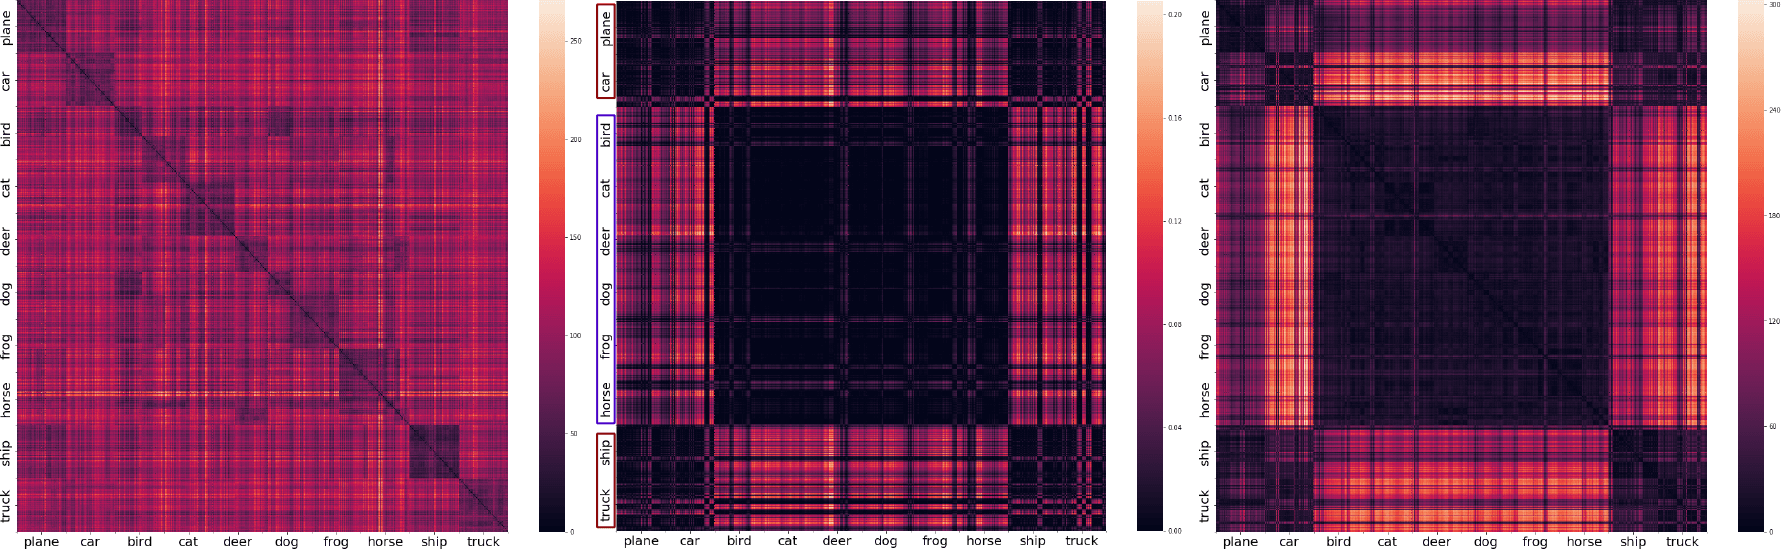
\includegraphics[width = \linewidth]{\imgpath/mse_matrices.png}
  \end{center}
  \caption{Representational similarity matrices of All-CNN trained on CIFAR-10 with (left) standard categorical cross-entropy, (middle) the invariance loss defined in Equation~\ref{eq:invariance-daug_class_objective} and (right) the invariance loss plus a categorical-cross entropy term. In the models trained with invariance losses, meaningful hierarchical clusters (animals vs. vehicles) emerge.}
  \label{fig:invariance-mse_matrices}
\end{figure}

In an additional effort to further understand the learnt representations without the limitation of the low accuracy on 10 classes, we created a subset of CIFAR-10 with the images of cars and dogs only, that is a binary classification problem. This data set could be classified correctly with high accuracy. In Figure~\ref{fig:invariance-2d_representations}, we see that in the model trained with the invariance objective most examples of the two classes are separated by a larger margin than in the baseline model, where the clusters of the two classes are closer to each other.

\begin{figure}[ht]
  \centering
  \begin{subfigure}{0.4 \linewidth}
      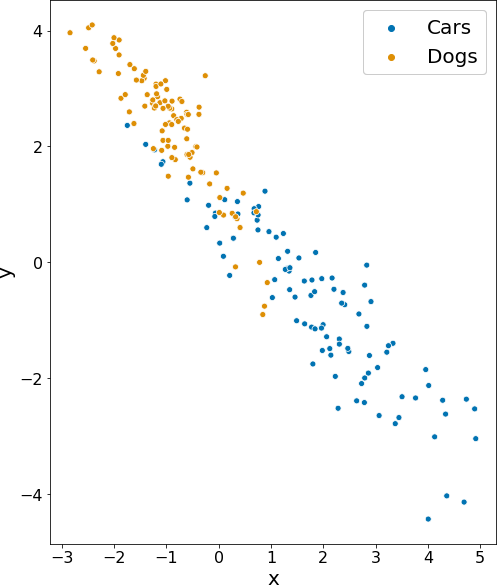
\includegraphics[width = \linewidth]{\imgpath/2drepr_noinv.png}
      \caption{Baseline model}
  \end{subfigure}
  \begin{subfigure}{0.4 \linewidth}
      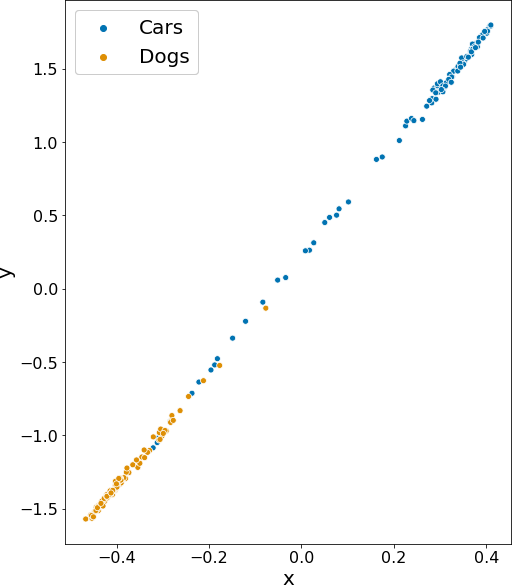
\includegraphics[width = \linewidth]{\imgpath/2drepr_inv.png}
      \caption{Invariance model}
  \end{subfigure}
  \caption{Representations of the test \textit{CIFAR-2} (cars and dogs) examples along the two principal components of the top layer representations of All-CNN.}
  \label{fig:invariance-2d_representations}
\end{figure}

Finally, we evaluated the adversarial robustness of the models. We had hypothesised that one of the reasons for adversarial vulnerability is that models optimised for categorisation only are highly unconstrained, with no specification of how the features should be. Therefore, the model focuses on learning any features that allows for linearly separable classes at the output of the network \citep{malhotra2020bioconstraints}. This has been shown to be prone to adversarial vulnerability, that is small perturbations largely affect the classification. In contrast, our invariance objective can be seen as the opposite strategy. It specifies how the features should be---increasingly invariant to identity-preserving transformations and relatively invariant within object classes---and expects good classification as a by-product. This could improve the sensitivity to adversarial perturbations and is what our results in Table~\ref{tab:invariance-adversarial_robustness} suggest: the model trained with the invariance objectives is remarkably more robust that the baseline models, without sacrificing performance.

\begin{table}[htb]
    \begin{center}
    \begin{tabular}{rcc}
                & Baseline (only cat.)  & Only invariance \\
        \hline
        Clean examples                 & 98.9~\% & 98.7~\%\\
        Attack: PGD $\varepsilon=0.03$  & 7.6~\%  & 62.0~\%\\
        Attack: FGSM $\varepsilon=0.03$ & 31.5~\% & 88.5~\%\\
    \end{tabular}
    \end{center}
    \caption{Adversarial robustness of the baseline (only categorisation) and invariance models trained on \textit{CIFAR-2}. Without any adversarial training, the model trained with the invariance objective only is highly robust to adversarial perturbations, in contrast to the standard, categorisation model.}
\label{tab:invariance-adversarial_robustness}
\end{table}

\section{Discussion}
\label{sec:invariance-discussion}
In this chapter, we have first proposed an invariance score that assesses the robustness of the features learnt by a neural network towards the identity-preserving transformations typical of common data augmentation schemes (see Equation~\ref{eq:invariance-invariance}). Intuitively, the more similar the representations of transformations of the same image, with respect to other images in a data set, the higher the data augmentation invariance score. The data augmentation score is meaningful in that the transformations performed by perceptually plausible data augmentation schemes---which we consider here exclusively---are motivated by human visual perception and coincide largely with the transformations to which the higher visual cortex is invariant.

Using this score, we have analysed the representations learnt by three popular neural network architectures---All-CNN, WRN and DenseNet---trained on image object recognition tasks---CIFAR-10 and Tiny ImageNet. The analysis revealed that their features are less invariant than commonly assumed, despite sufficient exposure to matching image transformations during training. In most cases, the representational invariance did not even increase with respect to the original pixel space. This property is fundamentally different to the primate ventral visual stream, where neural populations have been found to be increasingly robust to changes in view or lighting conditions of the same object \citep{dicarlo2007untangling}.

Taking inspiration from this property of the visual cortex, we have proposed a label-free objective to encourage learning more robust features, using data augmentation as the framework to perform identity-preserving transformations on the input data. We constructed mini-batches with $M$ augmented versions of each image and modified the loss function to maximise the similarity between the activations of the same seed images, as compared to other images in the batch. Aiming to approximate the observations in the biological visual system, higher layers were set to achieve exponentially more invariance than the early layers. An interesting avenue for future work will be to investigate whether this increased robustness also allows for better modelling of neural data.

Data augmentation invariance effectively produced more robust representations, unlike standard models optimised only for object categorisation, at little or no cost in classification performance and with an affordable, slight increase (10~\%) in training time. Ideally, object recognition models should be reasonably invariant to all the transformations of the objects to which human perception is also invariant. Data augmentation is just an approximation to analyse and encourage invariance to a set of transformations that can be applied on still, 2D images. Future work should analyse the invariance of models trained with video \citep{taylor2010spatiotemporal} and even 3D data \citep{achlioptas20183d}.

These results provide additional empirical evidence that deep supervised models optimised only according to the standard categorisation objective---the categorical cross-entropy between the true object labels and the model predictions---learn discriminative but non-robust features. This is likely due to their large capacity to learn discriminative features in too unconstrained a setting \citep{geirhos2020shortcutlearning, malhotra2020bioconstraints}, which has been recently suggested to be at the source of adversarial vulnerability \citep{ilyas2019advfeatures}.

In order to explore whether getting rid of the categorisation objective can produce features more aligned with our intuitions from visual perception, less vulnerable to adversarial perturbations and potentially more similar to the brain representations, we proposed to replace the categorical cross-entropy with purely invariance objectives. In particular, we combined layer-wise data augmentation invariance with class-wise invariance, which encourages similarity of the features from images of the same class. Although our preliminary experiments did not succeed at achieving competitive categorisation performance, we made interesting observations in our analysis.

First, training with invariance objectives yields representations that are clustered hierarchically, while the dissimilarity matrix of the standard model is fairly homogeneous. Remarkably, the main clusters formed through invariance learning correspond to the animate and inanimate classes, a separation consistently observed in the primate visual cortex \cite{kriegeskorte2008manandmonkey, bao2020itmaps}. Furthermore, we trained a model on a binary classification task using invariance objectives only and found that the adversarial vulnerability is very low, in contrast to categorisation models, which exhibit very high sensitivity to adversarial perturbations. While these conclusions are still speculative, they set a promising path for future research on alternative objective functions that encode inductive biases from visual perception and biological vision.

\chapterbibliography
}
